\documentclass[../main/git_course_main.tex]{subfiles}
\begin{document}

\setcounter{chapter}{0}
\chapter{Introduction to version control}

\section{Acknowledgements}

This material has been written with support from PlantLink, a research network for plant science in southern Sweden.

Many thanks to Ellen Sunström for providing extensive proof-reading.

%
% Johan Philipsson and Daniel Alm Grundström has contributed greatly to this material by supplying a never-ending input
% of opinions on Git and this material.
%
% Ellen Sunström has performed proof-reading.

% Thanks to Johan and Danne for never-ending input
% Thanks to Ellen for proof-reading
% Acknowledge the great web-page used as a basis

\section{Welcome}

Welcome to this introduction to version control and the version control software "Git" in particular. This material is geared towards bioinformaticians and puts an emphasis on parts
of Git that are particularly useful when doing bioinformatics, but it also aims to give a general understanding of version control, how to use Git and a bit of insight into how Git works internally.

\section{The structure of this document}

% Mention:
% Colored boxes
% Format for command introduction
% Illustrations

Each chapter is divided into three parts:

\begin{itemize}
	\item The reading part - Where the concepts are introduced together with demonstrations of the commands.
	\item The exercise part - Where the concepts are applied.
	\item The recap part - Where you can check and reinforce your understanding of the introduced concepts and commands.
\end{itemize}

In the text, you will encounter the following types of colored boxes:

\begin{figure}[h!]
\begin{codebox}
\vspace{10pt}
Command line examples are written within gray boxes. 
\begin{lstlisting}
$ Lines starting with "$" are commands run in the terminal
# Lines starting with "#" are comments
Other lines are output received when running the commands
\end{lstlisting}
\end{codebox}
\end{figure}

\begin{figure}[h!]
\begin{tcolorbox}[colback=red!5,colframe=red!40!black,title=Note]
Important notes and comments about potential pitfalls are shown in red boxes.
\end{tcolorbox}
\end{figure}

\begin{figure}[h!]
\begin{tcolorbox}[colback=blue!5,colframe=blue!40!black]
\verb$git add [-A] <path>$ \\

Git commands are introduced in blue boxes. Optional arguments
are shown within square brackets. Input arguments (strings, paths) are shown
in angular brackets. \\

In the example above, the \verb$[-A]$ indicates
that the command can take an \verb$-A$ flag which doesn't require an input argument. If the flag would have taken an argument, it would have been shown as: \verb$[-A <argument>]$. The command requires an input path.
\end{tcolorbox}
\end{figure}

\subsection{Visualizing Git}

This material makes frequent use of the kind of visualization shown in Figure \ref{fig:visualize_files_and_repo}. In this case it shows both the file tree (left), and the state of the \verb$repository$ which stores the history of the files (right). The file tree and the repository will be explained in more detail in the next chapter.

\begin{figure}[h!]
	\centering
	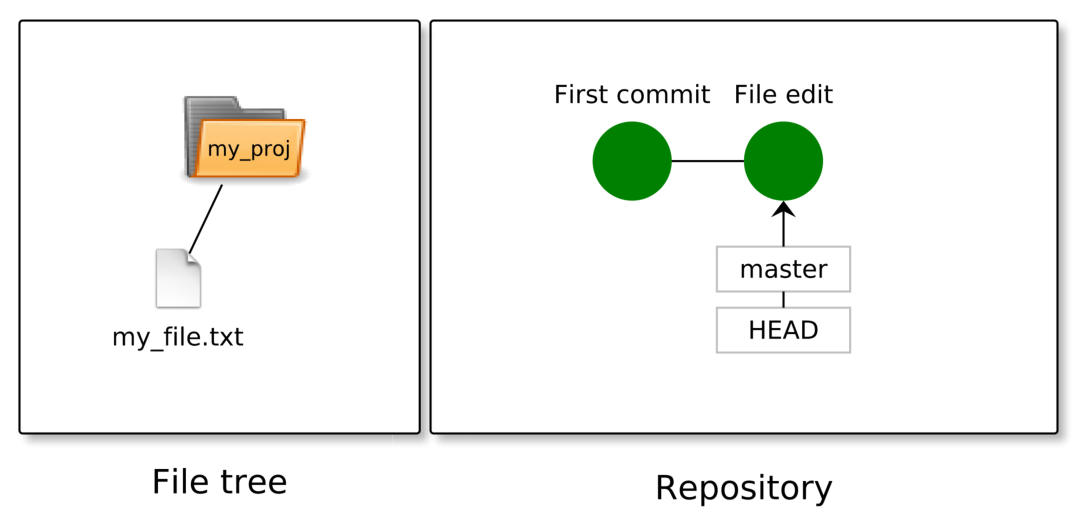
\includegraphics[width=0.8\textwidth]{../visualizations/chapter1/c11_visualize_file_system_and_repository.pdf}
	\caption{Example visualization of the file system and the repository}
	\label{fig:visualize_files_and_repo}
\end{figure}

We will also sometimes visualize a third component of Git - the \verb$stage$ (also called the \textit{index}). The stage is used as a gathering-place for file edits which are to be stored in the history. An example of this is shown below in Figure \ref{fig:visualize_stage} where \verb$my_file.txt$ has been newly created, and \verb$other_file.py$ has been edited. This will also be further explained in the following chapter.

\begin{figure}[h!]
	\centering
	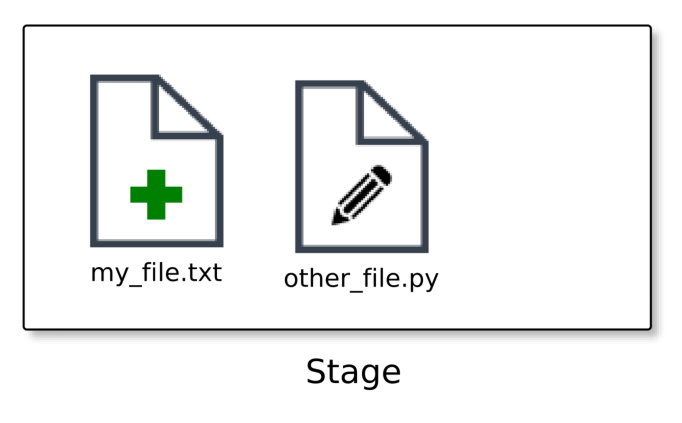
\includegraphics[width=0.6\textwidth]{../visualizations/chapter1/c12_demonstration_of_the_stage.pdf}
	\caption{Example visualization of the stage}
	\label{fig:visualize_stage}
\end{figure}

\section{What is version control?}

% Keep this brief

% Points to include in this chapter:
% - We keep track of all changes made to a file or a set of files
% - It allows us to later review specific versions
% - It also allows us to review what changes that has been done to a specific file
% - It is also a structured system giving multiple people a clear system for working with the same set of files

% Go through some more concepts and terms too here (repository, remote, commit)

\begin{figure}[h!]
\begin{verbatim}
"Version control is a system that records changes to a file or set of files 
 over time so that you can recall specific versions later"
- Pro Git (book)
\end{verbatim}
\end{figure}

A version control system keeps track of all the changes that you make within a designated directory, called the \verb$repository$. It allows you to recall previous versions of your files at a later time-point.

Repositories hosted in a version control system often have a central repository hosted on a server computer, called the \verb$remote$. This repository can be accessed from any computer with access rights. GitHub is a popular service providing remote hosting. More on this in Chapter 5.

The version control system provides a structured way of saving states of the file tree in the form of \verb$commits$. A commit contains a snapshot of the repository in a particular state. \\

There are many different version control systems. Here, we will be using Git. Git was initially conceived by Linus Torvald, the creator of the Linux kernel, 
and was developed by the Linux kernel developers. Git is currently one of the most widely used version control systems. Examples of other popular version control systems are Subversion (SVN) and Mercurial.

\section{Why use version control?}

%\begin{itemize}
%	\item Remove the need for the Abominable Commented Code Chunks
%	\item Easy back-tracking of errors in non-working versions
%	\item Reproducible research - Easier to keep track of used versions
%	\item A clear master document - Avoid the copy hell
%	\item Essential for any type of code teamwork
%	\item Clear history of all changes performed for the project
%\end{itemize}
%
%\subsection{Why use version control when I can use Dropbox?}

A version control system can serve many different purposes. 
In this material, it will be presented from the perspective of how it can be useful to a bioinformatician.

\begin{description}
\item[Reproducible research] It is not uncommon for bioinformaticians to have many copies of a particular script laying around in different locations, often in different versions. In order to be able to reproduce the analysis at a later stage, it is crucial that you later are able to re-run the exact same version of the code.
Git helps you with this as you:
	
\begin{enumerate}
	\item Can refer to the exact state of the code used. Git provides the ability to tag commits to easily keep track of important versions.	
	\item Have a central place for your code - You know exactly where to look for the different versions.
\end{enumerate}
	
\item[Easy back-tracking of errors] When you introduce bugs in your code, or accidentally remove an important paragraph, you can always back-track the changes made since the last working version. 

\item[Clear history of tasks] By looking at the history of commit messages, you get a clear overview of of the changes that have been made in the project at which times. This also allows for the pinpointing of changes made at particular points in time.

\item[Essential for code teamwork] If multiple people are working on the same source code, a version control system is a must. It provides a structured way
of implementing changes from different users, even when the changes are done on the same set of files.

\item[Code clarity] As all your previously saved code is stored within the history of the version control system, there is no longer any need to keep unused code which 'might come to use later'.
\end{description}

\subsection{Downsides to Git}

Git is useful in many ways, but as with all tools, the benefits come at a cost. Use your judgement to decide on when the benefits outweight the costs for you.

\begin{description}
\item[Learning curve] It is a new system to learn and understand. The basic commands are relatively easy to pick up, but it takes some effort to be able to use Git fluently outside the basic commands. Hopefully this material can help you with that!
\item[Another layer of complexity] It introduces another step into your workflow. This usually means running a few more commands per working-session, but can be more complex when running into problems.
\item[Geared for raw text] Version control systems like Git are designed to work with raw text. Git is able to keep track of binary files, but unable to track exact changes - it stores the full versions of the binary. It is often not a good idea to track binary files in Git.
\end{description}

\section{Why understand Git?}

One goal with this material is to give you some insight into how Git structures things internally and what happens when you run the different commands.
Often, one can simply run the commands without understanding the inner workings of Git, but some knowledge of the inner workings makes it much more straight-forward to debug errors and perform more complex tasks.

But, there is a lot going on inside the Git system which is outside the scope of a one-day course. If you have the time and the interest of digging deeper, you can take a look at the book \textit{Git from the bottom up} by John Wiegley. A web version of the book can be found at the following link: \\

\url{jwiegley.github.io/git-from-the-bottom-up}

\newpage
\section{Exercises}

The exercises in this material give you the opportunity to get hands-on practice with the introduced concepts. They closely follow the material. If you get stuck, you can usually find the answer in the text of the chapter.

Some of the exercises are marked with asterisks (*). Those are more challenging and/or time consuming exercises. If you are short on time, skip those on the first run-through. If you have the time - Do them. They will help you dig deeper into the introduced concepts.

\subsection{How to get help}

\begin{enumerate}
\item Make sure that you have a working version of Git running on your computer. Running the command \verb$git$ by itself should result in a number
of commonly used commands.

\begin{codebox}
\begin{lstlisting}
$ git
\end{lstlisting}
\end{codebox}

We will go through a number of these commands.
If you instead got an error message telling you that the command wasn't found, Git is likely not properly installed on your computer.
You will need to get Git running before proceeding.

\item To find out more about a Git command, type out the command (example: \verb$git add$) followed by the \verb$-h$ flag. 
If you want to get information about the \verb$git add$ command, you could type the following:

\begin{codebox}
\begin{lstlisting}
$ git add -h
\end{lstlisting}
\end{codebox}

To open the manual pages for a command, use the \verb$--help$ flag. This opens the manual page in \verb$less$.
(You exit \verb$less$ by pressing \verb$q$).

\begin{codebox}
\begin{lstlisting}
$ git add --help
\end{lstlisting}
\end{codebox}

\end{enumerate}

\subsection{Get used to finding help (*)}

\begin{enumerate}
\item Read the description in the help-pages for the following commands:

\begin{itemize}
	\item \verb$git init$
	\item \verb$git status$
	\item \verb$git add$
	\item \verb$git commit$
\end{itemize}

We will work with these commands in the coming chapter.

\end{enumerate}

\newpage
\section{Recap}

Every chapter ends with a recap of the introduced commands and concepts. Make sure that you have a good grasp of both the meaning of the commands 
and the different concepts.

\subsection{Concepts}

\begin{itemize}
\item How can Git be useful for you as a bioinformatician?
\item What are the potential troubles and limitations of Git?
\end{itemize}

\subsection{Commands}

\begin{itemize}
	\item \verb$git <command> -h$ \\\\
	Print brief information about a Git command to the terminal.
	\item \verb$git <command> --help$ \\\\
	Open the manual page for the command in \verb$less$.
\end{itemize}


\end{document}
